\newcommand{\svcourse}{CST Part IA: Introduction to Probability}
\newcommand{\svnumber}{1}
\newcommand{\svvenue}{Churchill, Room TBD}
\newcommand{\svdate}{2022-05-14}
\newcommand{\svtime}{11:00}
\newcommand{\svuploadkey}{PO5ogKIM8KQA22FZS8IAf8gxA8XKi19jxIBVHIfFZ+3GCBXuNUXS9lVN6bNYjxM/}

\newcommand{\svrname}{Mr Matthew Ireland}
\newcommand{\jkfside}{twoside}
\newcommand{\jkfhanded}{right}

\newcommand{\studentname}{Harry Langford}
\newcommand{\studentemail}{hjel2@cam.ac.uk}


\documentclass[10pt,\jkfside,a4paper]{article}

\input{../../template/includes.tex}
% DO NOT add \usepackage commands here.  Place any custom commands
% into your SV work files.  Anything in the template directory is
% likely to be overwritten!

\usepackage{fancyhdr}

\usepackage{lastpage}       % ``n of m'' page numbering
\usepackage{lscape}         % Makes landscape easier

\usepackage{verbatim}       % Verbatim blocks
\usepackage{epsfig}         % Embed encapsulated postscript
\usepackage{array}          % Array environment
\usepackage[nolinks]{qrcode}         % QR codes
\usepackage{enumitem}       % Required by Tom Johnson's exam question header

\usepackage{hhline}         % Horizontal lines in tables
\usepackage{siunitx}        % Correct spacing of units
\usepackage{amsmath}        % American Mathematical Society
\usepackage{amssymb}        % Maths symbols
\usepackage{amsthm}         % Theorems

\usepackage{ifthen}         % Conditional processing in tex

\usepackage[top=3cm,
            bottom=3cm,
            inner=2cm,
            outer=5cm]{geometry}

% PDF metadata + URL formatting
\usepackage[
            pdfauthor={\studentname},
            pdftitle={\svcourse, SV \svnumber},
            pdfsubject={},
            pdfkeywords={9d2547b00aba40b58fa0378774f72ee6},
            pdfproducer={},
            pdfcreator={},
            hidelinks]{hyperref}

\renewcommand{\headrulewidth}{0.4pt}
\renewcommand{\footrulewidth}{0.4pt}
\fancyheadoffset[LO,LE,RO,RE]{0pt}
\fancyfootoffset[LO,LE,RO,RE]{0pt}
\pagestyle{fancy}
\fancyhead{}
\fancyhead[LO,RE]{{\bfseries \studentname}\\\studentemail}
\fancyhead[RO,LE]{{\bfseries \svcourse, SV~\svnumber}\\\svdate\ \svtime, \svvenue}
\fancyfoot{}
\fancyfoot[LO,RE]{For: \svrname}
\fancyfoot[RO,LE]{\today\hspace{1cm}\thepage\ / \pageref{LastPage}}
\fancyfoot[C]{\qrcode[height=0.8cm]{\svuploadkey}}
\setlength{\headheight}{22.55pt}

\ifthenelse{\equal{\jkfside}{oneside}}{

 \ifthenelse{\equal{\jkfhanded}{left}}{
  % 1. Left-handed marker, one-sided printing or e-marking, use oneside and...
  \evensidemargin=\oddsidemargin
  \oddsidemargin=73pt
  \setlength{\marginparwidth}{111pt}
  \setlength{\marginparsep}{-\marginparsep}
  \addtolength{\marginparsep}{-\textwidth}
  \addtolength{\marginparsep}{-\marginparwidth}
 }{
  % 2. Right-handed marker, one-sided printing or e-marking, use oneside.
  \setlength{\marginparwidth}{111pt}
 }

}{
 % 3. Alternating margins, two-sided printing, use twoside.
}

\setlength{\parindent}{0em}
\addtolength{\parskip}{1ex}

% Exam question headings, labels and sensible layout (courtesy of Tom Johnson)
\setlist{parsep=\parskip, listparindent=\parindent}
\newcommand{\examhead}[3]{\section{#1 Paper #2 Question #3}}
\newenvironment{examquestion}[3]{
    \examhead{#1}{#2}{#3}\setlist[enumerate, 1]{label=(\alph*)}\setlist[enumerate, 2]{label=(\roman*)}
    \marginpar{\qrcode{https://www.cl.cam.ac.uk/teaching/exams/pastpapers/y#1p#2q#3.pdf}}
    \marginpar{\footnotesize \url{https://www.cl.cam.ac.uk/teaching/exams/pastpapers/y#1p#2q#3.pdf}}
}{}



\newcommand{\dfa}{\textit{DFA} }
\newcommand{\nfa}{\textit{NFA} }
\newcommand{\nfae}{\textit{NFA}$^\varepsilon$ }
\newcommand{\andautomaton}{\textit{And}$(M_1, M_2)$ }

\usepackage{tikz}

\usetikzlibrary{arrows,shapes,automata,petri,positioning,calc}

\tikzset{
    place/.style={
        circle,
        thick,
        draw=black,
        fill=lightgray!20,
        minimum size=10mm,
    },
        state/.style={
        circle,
        thick,
        minimum size=10mm,
    },
}

\begin{document}

\section*{4. Regular Languages:}

\begin{enumerate}

\item Why can’t the automaton \textit{Star}($M$) used in step (iv) of the proof of part (a)
of Kleene’s Theorem be constructed simply by taking $M$, making its start state the only
accepting state and adding new $\varepsilon$-transitions back from each old accepting state 
to its start state?

If we add new $\varepsilon$-transitions back from each old accepting state to the start state 
and make the start state accepting then the resulting automaton will accept a language which 
is a superset of the language accepted by the previous automaton (\dag). However it is not necessarily 
equal since it is possible for automatons to return to their start state without being 
accepted.

Consider the minimal counterexample $M = a^*b$. Here is a diagram of the \dfa $M$:

\begin{center}
\begin{tikzpicture}[node distance=1.5cm,>=stealth',auto, every place/.style={draw}]
\node [state, place] (q0) {$q_0$};
\node [state, place, initial text =, accepting by double] (q1) [right = of q0] {$q_1$};
\node [state, place] (q2) [right = of q1] {$q_2$};
\coordinate [node distance=1cm, left of = q0] (left);
\draw [->] (left) -- (q0);
\path [->] (q0) edge [loop above] node {$a$} ();
\path [->] (q0) edge [bend left] node {$b$} (q1);
\path [<-] (q2) edge [bend left] node {$a$} (q1);
\path [->] (q1) edge [bend left] node {$b$} (q2);
\path [->] (q2) edge [loop above] node {$a$} ();
\path [->] (q2) edge [loop below] node {$b$} ();
\end{tikzpicture}
\end{center}

If we add an epsilon transition from $q_1$ to $q_0$, make $q_0$ accepting and $q_1$ non-accepting 
then the \nfae formed will now also accept $a^*$. Consider specifically $a$. It is easy to 
see that $a$ is accepted by this \nfae while it is not accepted in \textit{Star}$(M)$. 
So this \nfae is not \textit{Star}$(M)$.

\begin{center}
\begin{tikzpicture}[node distance=1.5cm,>=stealth',auto, every place/.style={draw}]
\node [state, place, initial text =, accepting by double] (q0) {$q_0$};
\node [state, place] (q1) [right = of q0] {$q_1$};
\node [state, place] (q2) [right = of q1] {$q_2$};
\coordinate [node distance=1cm, left of = q0] (left);
\draw [->] (left) -- (q0);
\path [->] (q0) edge [loop above] node {$a$} ();
\path [->] (q1) edge [bend left] node {$\varepsilon$} (q0);
\path [->] (q0) edge [bend left] node {$b$} (q1);
\path [<-] (q2) edge [bend left] node {$a$} (q1);
\path [->] (q1) edge [bend left] node {$b$} (q2);
\path [->] (q2) edge [loop above] node {$a$} ();
\path [->] (q2) edge [loop below] node {$b$} ();
\end{tikzpicture}
\end{center}

\begin{enumerate}[label=(\dag)]

\item Assume that the previous automaton is in an accepting state.

Consider the automaton formed by adding $\varepsilon$-transitions from old accepting states 
to the start state and making the start state the only accepting state.

The input leaves the new automaton in one of the old accepting states. However since there 
is a $\varepsilon$-transition to an accepting state, the new automaton is now in an accepting 
state.

So the language accepted by the new automaton is a superset of the language accepted by the old 
automaton.

\end{enumerate}

\item Construct an \nfae $M$ satisfying $L(M) = L((\epsilon|b)^*aab^*)$.

\begin{center}
\begin{tikzpicture}[node distance=1.5cm,>=stealth',auto, every place/.style={draw}]
\node [state, place] (q0) {$q_0$};
\node [state, place] (q1) [right = of q0] {$q_1$};
\node [state, place, initial text =, accepting by double] (q2) [right = of q1] {$q_2$};
\coordinate [node distance=1cm, left of = q0] (left);
\draw [->] (left) -- (q0);
\path [->] (q0) edge [loop above] node {$b$} ();
\path [->] (q0) edge [bend left] node {$a$} (q1);
\path [->] (q1) edge [bend left] node {$a$} (q2);
\path [->] (q2) edge [loop above] node {$b$} ();
\end{tikzpicture}
\end{center}

\item Show that any finite set of strings is a regular language.

Let $S$ be an arbitrary finite set of strings over the alphabet $\Sigma$.

By definition a string is a finite sequence of symbols in the alphabet $\Sigma$.

\[
\begin{split}
\forall s \in S.& s \textit{ finite} \Longrightarrow \\
\forall s \in S.& \{s\} = L(s) \Longleftrightarrow \\
\forall s \in S.& \exists \dfa \text{ } d. \{s\} = L(d) \text{ using Kleene's Theorem} \\
\end{split}
\]

Now consider the set of \textit{DFA}'s $D$ such that every $d \in D$ recognises a unique 
$s \in S$.

Consider now the \nfae which has a new start state and $\varepsilon$-transitions to 
the start state of every $d \in D$. This \nfae must accept all strings which are accepted 
by any $d \in D$. So this \nfae must accept all strings $s \in S$.

Since there exists a \nfae which accepts $S$; by Kleene’s Theorem $S$ is a regular language.
Since $S$ was arbitrary we can conclude that any finite set of strings is a regular language.

\item Use the construction given in the proof of part (b) of Kleene’s Theorem to find
a regular expression for the \dfa $M$ whose state set is \{0, 1, 2\}, whose start state is 0, whose
only accepting state is 2, whose alphabet of input symbols is $\{a, b\}$, and whose next-state
function is given by the following table.

\begin{center}
\begin{tabular}{c|c c}
$\delta$ & $a$ & $b$ \\
\hline
0 & 1 & 2 \\
1 & 2 & 1 \\
2 & 2 & 1 \\
\end{tabular}
\end{center}

Here is a diagram of the \dfa $M$:

\begin{center}
\begin{tikzpicture}[node distance=1.5cm,>=stealth',auto, every place/.style={draw}]
\node [state, place] (q0) {0};
\node [state, place] (q1) [right = of q0] {1};
\node [state, place, initial text =, accepting by double] (q2) [below right = 1cm of q0] {2};
\coordinate [node distance=1cm, left of = q0] (left);
\draw [->] (left) -- (q0);
\path [->] (q0) edge [bend left] node {$a$} (q1);
\path [<-] (q2) edge [bend left] node {$b$} (q0);
\path [->] (q1) edge [bend left] node {$a$} (q2);
\path [->] (q1) edge [loop above] node {$b$} ();
\path [->] (q2) edge [loop below] node {$a$} ();
\path [->] (q2) edge [bend left] node {$b$} (q1);
\end{tikzpicture}
\end{center}

Part (b) of Kleene's Theorem has four parts:

\begin{itemize}

\item $R^k_{ij}$ is regular expression for all paths from $i$ to $j$ which do not pass 
through any vertices $> k$.

\item $R^0_{ij}$ is the union of all edges from $i$ to $j$.

\item $R^k_{ij} = R^{k-1}_{ik}(R^{k-1}_{kk})^*R^{k-1}_{kj}$

\item $R^n_{0n}$ is the language accepted by the automata.

\end{itemize}

\begin{center}
\begin{tabular}{c|c|c|r l}
i & j & k & \multicolumn{2}{c}{$R^k_{ij}$} \\
\hline
0 & 0 & -1 & & $\varepsilon$ \\
0 & 1 & -1 & & $a$ \\
0 & 2 & -1 & & $b$ \\
1 & 0 & -1 & & $\emptyset$ \\
1 & 1 & -1 & & $b|\varepsilon$ \\
1 & 2 & -1 & & $a$ \\
2 & 0 & -1 & & $\emptyset$ \\
2 & 1 & -1 & & $b$ \\
2 & 2 & -1 & & $a|\varepsilon$ \\
0 & 0 & 0 & $\varepsilon\varepsilon^*\varepsilon|\varepsilon$ &= $\varepsilon$ \\
0 & 1 & 0 & $\varepsilon\varepsilon^*a|a$ &= $a$ \\
0 & 2 & 0 & $\varepsilon\varepsilon^*b|b$ & $b$ \\
1 & 0 & 0 & $\emptyset\varepsilon^*\varepsilon|\emptyset$ &= $\emptyset$ \\
1 & 1 & 0 & $\emptyset\varepsilon^*a|b|\varepsilon$ &= $b|\varepsilon$ \\
1 & 2 & 0 & $\emptyset\varepsilon^*b|a$ &= $a$ \\
2 & 0 & 0 & $\emptyset\varepsilon^*\varepsilon|\emptyset$ &= $\emptyset$ \\
2 & 1 & 0 & $\emptyset\varepsilon^*a|b$ &= $b$ \\
2 & 2 & 0 & $\emptyset\varepsilon^*\varepsilon|a|\varepsilon$ &= $a|\varepsilon$ \\
0 & 0 & 1 & $a(b|\varepsilon)^*\emptyset|\varepsilon$ &= $\varepsilon$ \\
0 & 1 & 1 & $a(b|\varepsilon)^*(b|\varepsilon)|a$ &= $ab^*$ \\
0 & 2 & 1 & $a(b|\varepsilon)^*a|b$ &= $ab^*a|b$ \\
1 & 0 & 1 & $(b|\varepsilon)(b|\varepsilon)^*\emptyset|\emptyset$ &= $\emptyset$ \\
1 & 1 & 1 & $(b|\varepsilon)(b|\varepsilon)^*(b|\varepsilon)$ &= $b^*$ \\
1 & 2 & 1 & $(b|\varepsilon)(b|\varepsilon)^*a|a$ &= $b^*a$ \\
2 & 0 & 1 & $b(b|\varepsilon)^*\emptyset|\emptyset$ &= $\emptyset$ \\
2 & 1 & 1 & $b(b|\varepsilon)^*(b|\varepsilon)|b$ &= $bb^*$ \\
2 & 2 & 1 & $b(b|\varepsilon)^*a|a|\varepsilon$ &= $b^*a|\varepsilon$ \\
0 & 2 & 2 & $(ab^*a|b)(b^*a|\varepsilon)^*(b^*a|\varepsilon)|(ab^*a|b)$ &= $(ab^*a|b)(b^*a)^*$ \\
\end{tabular}
\end{center}

So the regular expression which is equivalent to the \dfa is:
\[(ab^*a|b)(b^*a)^*
\]

\item If $M = (Q, \Sigma, \Delta, s, F)$ is an \nfa, let \textit{Not}($M$) be the 
\nfa $(Q, \Sigma, \Delta, s, Q / F)$ obtained from $M$ by interchaining the role of accepting 
and non-accepting states. Give an example of an alphabet $\Sigma$ and an \nfa $M$ with the 
set of input symbols $\Sigma$, such that $\{u \in \Sigma^*\ | u \notin L(M)\}$ is \textit{not} 
the same set as $L$(\textit{Not}($M$)).

Consider the \nfa $M$ with input alphabet $\Sigma = \{a\}$ which accepts only $\varepsilon$.

Here is a diagram of $M$:

\begin{center}
\begin{tikzpicture}[node distance=1.5cm,>=stealth',auto, every place/.style={draw}]
\node [state, place, initial text =, accepting by double] (q0) {$q_0$};
\end{tikzpicture}
\end{center}

Note that $M$ does not accept the string $a$ -- or more generally any string of the form 
$aa^*$, however my proof involves only $a$.

Consider now \textit{Not}$(M)$:

\begin{center}
\begin{tikzpicture}[node distance=1.5cm,>=stealth',auto, every place/.style={draw}]
\node [state, place] (q0) {$q_0$};
\end{tikzpicture}
\end{center}

\textit{Not}$(M)$ has no accepting states and so accepts no strings, namely $a$.

So:
\[
\begin{split}
a \notin L(M) &\wedge a \notin L(\textit{Not}(M)) \Longleftrightarrow \\
a \in \{u \in \Sigma^*| u \notin L(M)\} &\wedge a \notin a \in L(\textit{Not}(M)) \Longrightarrow \\
\{u \in \Sigma^*| u \notin L(M)\} &\neq L(\textit{Not}(M)) \text{ as required}
\end{split}
\]

\item Let $r = (a|b)^*ab(a|b)^*$. Find a complement for $r$ over the alphabet $\{a, b\}$, i.e. a 
regular epression $\sim r$ over the alphabet $\{a, b\}$ satisfying $L(\sim r) = \{u \in \{a, b\}^* | u \notin L(r)\}$.

\[
\sim r = b^*a^*
\]

\item Given \textit{DFA}s  $M_i = (Q_i, \Sigma, \delta_i, s_i, F_i)$ for $i = 1, 2$, let \textit{And}$(M_1, M_2)$ 
be the \dfa $(Q_1 \times Q_2, \Sigma, \delta, (s_1, s_2), F_1 \times F_2)$ where $\delta : (Q_1 \times Q_2) \times \Sigma \longrightarrow (Q_1 \times Q_2)$ is 
given by:
\[
\delta((q_1, q_2), a) = (\delta_1(q_1, a), \delta_2(q_2, a))
\]
for all $q_1 \in Q_1, q_2 \in Q_2$ and $a \in \Sigma$. Show that $L($\textit{And}$(M_1, M_2))$ is the 
intersection of $L(M_1)$ and $L(M_2)$.

I will show by induction that the state of \andautomaton after a string of length $n$, $s_n$ 
is equal to $(q_1, q_2)$ where $q_1$ is $M_1$'s 
state and $q_2$ is $M_2$'s state.

If $s = \varepsilon$:

Then all \textit{DFA}'s are in their start states. So the state of \andautomaton is $(s_1, s_2)$, the 
state of $M_1$ is $s_1$ and the state of $M_2$ is $s_2$. So the statement holds for $s = \varepsilon$.

\vspace{0.1cm}

Assume that the statement holds for some string $s_k$. 

Let $s_{k+1}$ be a string such that $s=s_kv$ where $v \in \Sigma$.
So the state of \andautomaton after string $s$ is $\delta((q_1, q_2), v) = (\delta_1(q_1, v), \delta_2(q_2, v))$, 
the state of $M_1$ after 
string $s$ is $\delta_1(q_1, v)$ and the state of $M_2$ after string $s$ is $\delta_2(q_2, v)$. 
So if the statement holds for some arbitrary string $s_k$ of length $k$ then it also holds for all 
strings $s_{k+1}$ of length $k+1$.

\vspace{0.1cm}

Since the statement holds for $s = \varepsilon$ and the statement holding for a string of length $k$ implies 
that it also works for a string of length $k + 1$.

So this implies that $\forall n \in \mathbb{N}$ after input $s_n$, the state of \andautomaton is equal to $(q_1, q_2)$ where $q_1$ is the 
state of $M_1$ and $q_2$ is the state of $M_2$.

The accepting states of \andautomaton are $(f_1, f_2)$ where $f_1 \in F_1, f_2 \in F_2$. By the proof above this 
means that \andautomaton is in an accepting state if and only if both $M_1$ and $M_2$ are in accepting states.

Hence $L(\textit{And}(M_1, M_2))$ is the intersection of $L(M_1)$ and $L(M_2)$.

\end{enumerate}

\subsection*{5. The Pumping Lemma:}

\begin{enumerate}

\item Consider
\[
L \triangleq \{c^ma^nb^n | m \geq 1 \wedge n \geq 0\} \cup \{a^mb^n | m, n \geq 0\}
\]
The notes show that this language has the pumping lemma property. Show that there is no
\dfa $M$ which accepts $L$. [\textit{Hint}: argue by contradiction. If there were such an $M$, consider
the \dfa $M_0$ with the same states as $M$, with alphabet of input symbols just consisting of $a$
and $b$, with transitions all those of $M$ which are labelled by $a$ or $b$, with start state 
$\delta_M(s_M, c)$ (where $s_M$ is the start state of $M$), and with the same accepting states as $M$. Show 
that the language accepted by $M'$ has to be $\{a^nb^n| n \geq 0\}$ and deduce that no such 
$M$ can exist].

Assume $L$ is a regular language.

This implies that there is a \dfa D which recognises $L$. \\
Since $D$ recognises $L$, it must recognise $\{c^ma^nb^n\}$ (since this is a subset of $L$). \\
Now consider a \nfa which contains only the $a, b$ transitions in $D$. \\
Since the \dfa recognises $\{c^ma^nb^n\}$, without $c$ transitions the \nfa will recognise $a^nb^n$. \\
However by the pumping lemma, $a^nb^n$ is not a regular language. By Kleene’s Theorem, this is 
equivalent to saying there is no \nfa which recognises $a^nb^n$. \\
This is a contradiction. So our original assumption that $L$ is a regular language must be wrong. 

So $L$ is not a regular language.

\end{enumerate}

\begin{examquestion}{2021}{2}{10}

\begin{enumerate}

\item Consider the following \nfae, whose input alphabet is $\{a, b, c\}$.

\begin{center}
\begin{tikzpicture}[node distance=1.5cm,>=stealth',auto, every place/.style={draw}]
\node [state, place] (d) {$D$};
\node [state, place, initial text =, accepting by double] (f) [right = of d] {$F$};
\node [state, place] (e) [below = of d] {$E$};
\coordinate [node distance=1cm, left of = d] (left);
\draw [->] (left) -- (d);
\path [->] (d) edge [loop above] node {$a$} ();
\path [->] (d) edge [bend left] node {$a$} (e);
\path [<-] (e) edge node {$\varepsilon$} (d);
\path [->] (e) edge [bend left] node {$b$} (d);
\path [<-] (f) edge [bend left] node {$\varepsilon$} (e);
\path [->] (f) edge [loop right] node {$b$} ();
\path [stealth-] (d) edge [bend left] node {$a$} (f);
\end{tikzpicture}
\end{center}

\begin{enumerate}

\item For each of the two strings $abc$ and $bba$, state whether the automaton accepts it, 
with justification

The automaton does not accept either $abc$.

For $abc$ there is no transition for $c$ and so it enters an undefined state which is 
not in the set of accepting states.

The automaton does accept $bba$.

It can $\varepsilon$-transition to from D to E, then transition to D with $b$. Repeat that again.
Then transition to D using $a$. then $\varepsilon$-transition to E and $\varepsilon$-transition to F. 
This means that after $bba$, the automaton is in an accepting state and so $bba$ is accepted by 
the automaton.

\item Using the subset construction, produce the full unoptimized state transition table of 
an equivalent \dfa, \textit{listing its states in lexicographic order} (important!) and 
indicating the starting and accepting states.

\begin{center}
\begin{tabular}{c|c c c}
Q & a & b & c \\
\hline
$\emptyset$ & $\emptyset$ & $\emptyset$ & $\emptyset$ \\
\{D\} & \{D, E, F\} & \{D, E, F\} & $\emptyset$ \\
\{D, E\} & \{D, E, F\} & \{D, E, F\} & $\emptyset$ \\
\{D, E, F\} & \{D, E, F\} & \{D, E, F\} & $\emptyset$ \\
\{D, F\} & \{D, E, F\} & \{D, E, F\} & $\emptyset$ \\
\{E\} & \{D, E, F\} & \{D, E, F\} & $\emptyset$ \\
\{E, F\} & \{D, E, F\} & \{D, E, F\} & $\emptyset$ \\
\{F\} & \{D, E, F\} & \{F\} & $\emptyset$ \\
\end{tabular}
\end{center}

The starting state is $\{D, E, F\}$.

The accepting states are $\{D, E, F\}, \{D, F\}, \{E, F\}, \{F\}$

\item Give a regular expression, no longer than six symbols (metacharacters included), that 
describes the strings accepted by the automaton, together with an intuitive explanation for it. 
[\textit{Hint}: part (a)(ii) helps.]

Looking at the table in (a)(ii), note that the \dfa starts in an accepting state and that 
the \dfa will be in an accepting state after a transition iff it was in an accepting state 
before the transition and is passed either $a$ or $b$.

From this, I gather that any sequence of $a$'s and $b$'s will be accepted. 
The regular expression for this is given below:

\[
(a|b)^*
\]

So any string of the form $(a|b)^*$ will be accepted by the automaton..

\end{enumerate}

\item 

Consider language $L_1$ of strings over alphabet $\{0, 1\}$, defined inductively as follows
\[
\frac{}{00} \hspace{1cm} \frac{w}{1w} \hspace{1cm} \frac{w}{w1}
\]

\begin{enumerate}

\item Draw the diagram of a \dfa that recognises $L_1$ in no more than four states.

\begin{center}
\begin{tikzpicture}[node distance=1.5cm,>=stealth',auto, every place/.style={draw}]
\node [state, place] (q0) {$q_0$};
\node [state, place] (q1) [right = of q0] {$q_1$};
\node [state, place, initial text =, accepting by double] (q2) [right = of q1] {$q_2$};
\node [state, place] (q3) [below right = 1cm of q1] {$q_3$};
\coordinate [node distance=1cm, left of = q0] (left);
\draw [->] (left) -- (q0);
\path [->] (q0) edge [loop above] node {1} ();
\path [->] (q0) edge [bend left] node {0} (q1);
\path [->] (q1) edge [bend left] node {0} (q2);
\path [<-] (q3) edge [bend left] node {1} (q1);
\path [->] (q2) edge [loop above] node {1} ();
\path [->] (q2) edge [bend left] node {0} (q3);
\path [->] (q3) edge [loop above] node {1} ();
\path [->] (q3) edge [loop below] node {0} ();
\end{tikzpicture}
\end{center}

\item Considering the words in $L_1$ as unsigned binary numerals, let language $L_2$ of strings over 
$\{0, 1\}$ be the set of all and only the binary numerals obtained by adding 1 to any numeral in 
$L_1$ and removing any leading zeros.\\
NB: ``adding'' here means arithmetic addition, not string concatenation.\\
Produce a regular expression no longer than 11 symbols that recognizes $L_2$, with a 
clear and convincing explanation of how you derived it.

\[
L_2 = L((\varepsilon|1^*10)10^*)
\]

\begin{itemize}

\item By inspection: $L_1$ is the set of strings which are of the form $1^*001^*$. 

\item Adding one to a string $s \in L_1$ gives a string of the form $1^*010^*$.

\item 

If the number of ones preceding 00 was zero there will be a single leading zero to remove. 

This case gives strings of the form $10^*$

If the number of ones preceding 00 was nonzero then there are no leading zeros to remove. 

This case gives strings of the form $1^*1010^*$.

\item To form the regular expression which accepts the language $L_2$ we must take the union 
of these two regular expressions:

\[
10^*|1^*1010^* = (\varepsilon|1^*10)10^*
\]

So the regular expression which accepts the language $L_2$ is $(\varepsilon|1^*10)10^*$.

\end{itemize}

\end{enumerate}

\end{enumerate}

\end{examquestion}

\end{document}